%
% \section{Crear el Frontend}
% \label{sec:Crear el Frontend}
% TODO move to marco teorico

El frontend como ya se mencionó es la vista de la aplicación, es donde el usuario interactúa con la aplicación, en el presente proyecto se implementó usando \emph{Ember.JS}, el cual es un framework de desarrollo JavaScript orientado a crear Aplicaciones de Página Única, esto quiere decir que una vez que se carge la pagina la primera vez ya no se recargara la pagina como tal, en cambio se actualizará de acuerdo como el usuario interactúa con la aplicación.\\

Ya que el proyecto se enfocara en la creación de una aplicación web optimizada para su uso en celulares, es primordial que el ``look and feel'' de la aplicación sea lo más parecido a una aplicación móvil nativa, para lograr este efecto se utilizó \emph{ember-paper}, que ya trae implementado componentes (botones, listas, links, menús de navegación, etc.) con un comportamiento que emula a una aplicación móvil nativa.\\

% Para empezar esta tarea se procedió a instalar y configurar el framework de desarrollo Ember JS, que nos ayudará en la implementación del frontend de la aplicación o la capa que interactúa con el usuaria, y Express JS, el cual manejara el backend de la aplicación, básicamente se encarga de la lógica del sistema y la comunicación con la base de datos.\\

\emph{EmberJS} está basado en ``Convención sobre Configuración'', ya que la gran mayoría de los problemas con que uno se puede enfrentar a la hora de crear una aplicación web ya fueron resueltas por la comunidad de desarrollo, por lo tanto ya se llegó a un patrón o convención de cómo se debería resolver algún determinado problema, \emph{EmberJS} implementa y sugiere soluciones a problemas comunes, para que de esa forma el desarrollo no se enfoque  en resolver problemas ya resueltos (configuración) si no en implementar en la lógica del negocio de la aplicación, que al final es lo que le da valor al producto que queremos desarrollar y también para que si en un futuro otro desarrollador empieza a trabajar en el proyecto, sea capaz de entender la estructura y el diseño de la aplicación de forma sencilla. Por lo tanto nos enfocaremos en analizar cómo se resolvieron los problemas: de geolocalizar el lugar sobre un mapa, mostrar la ruta más corta dentro del campus Universitario, manejo de los usuario y como mostrar el reporte de los lugares más visitados.
% TODO move to marco teorico


% TODO movido a implementacion - iteracion 2
\subsection{Geolocalizar los Lugares}
\label{sub:fronted_lugares}

Un ``lugar'' tienen almacenada en la base de datos su posición georreferenciada, por lo tanto la aplicación necesita mostrar un lugar o geolocalizarlo sobre un mapa. Para resolver esta tarea se utilizó \emph{ember-leaflet}, una librería creada para manipular mapas y diseñada especialmente  para su implementación en dispositivos móviles.\\

Para instalar esta librería solo se necesita ejecutar el siguiente comando y posteriormente ya se puede empezar a utilizarla.\\

\begin{verbatim}
 $ ember install ember-leaflet
\end{verbatim}


En primer lugar para obtener la coordenada del ``lugar'', se necesita hacer un \emph{request} al API de la aplicación y este responde con la información del ``lugar'' en formato GeoJSON, dentro del \emph{controlador} de ember se procesa la información recibida para asignar los valores necesarios al \emph{template}, tal como se puede observar en el siguiente codigo, los atributos de \emph{lat} y \emph{lng} son la latitud y longitud respectivamente, la combinación de ambos datos es la locación donde se va a centrar la ubicación del renderizado del mapa. Se puede notar que el \emph{tag} $leaflet-map$ es un componente personalizado, perteneciente a \emph{ember-leaflet}, es donde se inicializa el mapa en este caso \emph{Open Street Maps}, como se puede apreciar en la figura \ref{fig:ember_leaflet}.


% \begin{center}
%   \begin{verbatim}
%     var maker = new google.maps.Marker({
%       position: new google.maps.LatLng( lat, lng  )
%       map: UMSS.map
%     });
%   \end{verbatim}
% \end{center}

\begin{verbatim}
  {{#leaflet-map lat=lat lng=lng zoom=zoom}}
    {{tile-layer url="http://{s}.tile.openstreetmap.fr/hot/{z}/{x}/{y}.png" }}
      {{#marker-layer location=location}}
        <h3>{{model.name}}</h3>
        {{model.description}} <br>
        <strong>telf:</strong> {{model.phone}} <br>
        <strong>piso </strong>#{{model.level}}
    {{/marker-layer}}
  {{/leaflet-map}}
\end{verbatim}


\begin{figure}[H]
      \begin{center}
        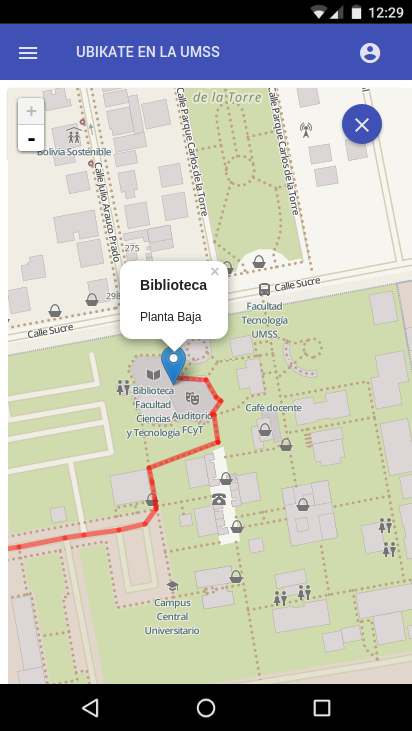
\includegraphics[width=0.5\textwidth]{ember_leaflet}

        % \caption{\emph{ember-leaflet} nos ayuda a desplegar un mapa y mostrar un \emph{punto} o \emph{lugar} con un \emph{marcador} y dibuja una línea de color rojo sobre el mapa.}
        \caption{ Mapa mostrado con la ayuda de \emph{ember-leaflet}}
        \label{fig:ember_leaflet}
        \caption*{Fuente: Elaboración propia.}
      \end{center}
\end{figure}

\emph{Ember-leaflet} se encarga de geolocalizar un punto georreferenciado sobre un mapa y también permite personalizarlo, por ejemplo se puede añadir un \emph{marcador}  y personalizarlo con el \emph{tag} $#marker-layer$ e incluir los demás datos obtenidos del backend, como se puede apreciar en la figura \ref{fig:baquita_place}.


\begin{figure}[H]
  \begin{center}
    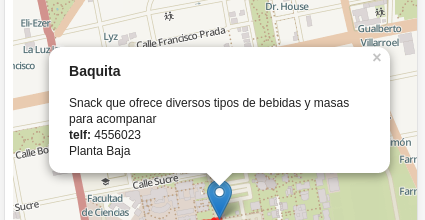
\includegraphics[width=0.8\textwidth]{iteration2/baquita_place}
    \caption{Tooltip con la información de un lugar.}
    \label{fig:baquita_place}
    \caption*{Fuente: Elaboración propia.}
  \end{center}
\end{figure}


% Para poder acceder a la anterior vista, es necesario en primer lugar seleccionarlo de una lista





% \begin{figure}[H]
%  \begin{center}
%    \caption{Vista de la lista de Lugares registrados en el sistema.}
%    \label{fig:places_index}
%    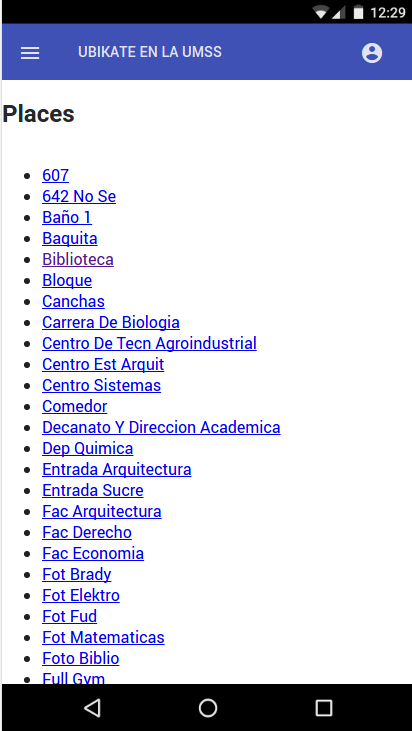
\includegraphics[width=0.5\textwidth]{iteration1/places_index}
%    \caption*{Fuente: Elaboración propia}
%  \end{center}
% \end{figure}


% \begin{figure}[H]
%  \begin{center}
%    \caption{Vista de la búsqueda de lugares a través de un cajón de búsqueda.}
%    \label{fig:places_search}
%    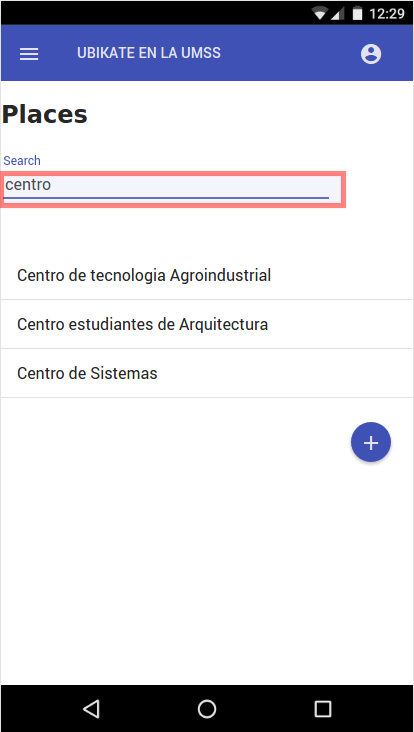
\includegraphics[width=0.5\textwidth]{iteration1/places_search}
%    \caption*{Fuente: Elaboración propia}
%  \end{center}
% \end{figure}


% Para implementar esta funcionalidad del sistema fue necesario utilizar las funcionalidad de Ember JS.
%
% \begin{verbatim}
%  {{#paper-item class="md-1-line" onClick=(transition-to 'places.show' place)}}
%      <div class="md-list-item-text">
%          <span>{{place.name}}</span>
%      </div>
%  {{/paper-item}}
% \end{verbatim}
%
%
% \begin{figure}[H]
%    \label{fig:place_show}
%    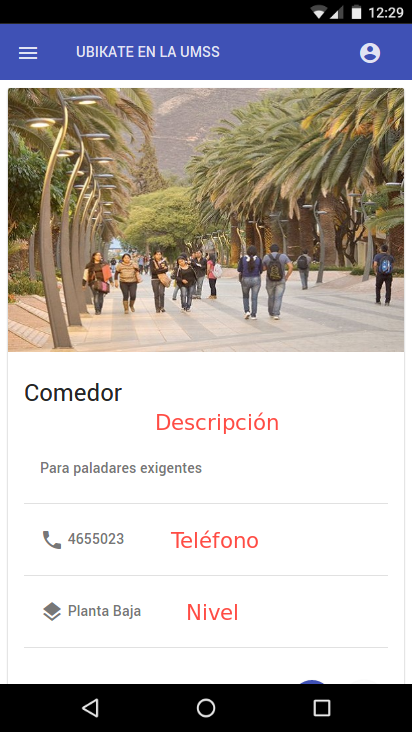
\includegraphics[width=0.5\textwidth]{iteration1/place_show}
%    \caption*{Fuente: Elaboración propia}
%  \end{center}
% \end{figure}

% movido a implementacion - iteracion 1





% movido a iteration 2
\subsection{Mostrar los Rutas}
\label{sub:Mostrar los Rutas}

Para mostrar la ruta óptima es necesario obtener de la base de datos un conjunto de datos en formato de latitud y longitud que conforman líneas, las cuales representan la ruta más corta, pero al final es solo un montón de números, sin mucho significado para el usuario, toda esta información es difícil de procesar y el usuario necesita información que sea fácil de entender y no existe mejor herramienta disponible para esta tarea que mostrar la \emph{ruta} de forma visual, esto quiere decir que se necesita mostrar la ruta sobre un \emph{mapa}, ya que en la aplicación se implementó \emph{ember-leaflet} para desplegar el mapa y mostrar un lugar, también se puede  mostrar más ruta más corta mediante una línea, a la que también se puede personalizar (la línea se muestra de color rojo).\\

A continuación se puede apreciar el \emph{request} que el frontend hace al API y  el objeto GeoJSON que es recibido, este objeto contiene la información geoespacial necesaria para ``dibujar'' la línea roja entre 2 puntos georeferenciados, uno de los puntos es donde se encuentra el usuario (\emph{sourceData}) y el otro punto es el lugar (\emph{targetData}).
% A continuación se puede apreciar el request al API

 % uno de los cuales es el lugar al que se quiere llegar y el otro es la ubicación actual del usuario. \\

\begin{verbatim}
  ENV.APP.API_HOST + '/api/v1/ways/route/' + sourceData.id + '/' + targetData.id;

  GET /api/v1/ways/route/930/77 200 276.217 ms - 3911

  $ curl http://localhost:3000/api/v1/ways/route/930/77 | python -m json.tool                                                       [3:04:52]
  % Total    % Received % Xferd  Average Speed   Time    Time     Time  Current
                                 Dload  Upload   Total   Spent    Left  Speed
100  3911  100  3911    0     0   161k      0 --:--:-- --:--:-- --:--:--  166k
{
    "features": [
        {
            "geometry": {
                "coordinates": [
                    [
                        -66.1467397848201,
                        -17.3935321732846
                    ],
                    [
                        -66.1467190789842,
                        -17.3935294725234
                    ]
                ],
                "type": "LineString"
            },
            "type": "Feature"
        },

\end{verbatim}
% /api/v1/ways/route/

Una vez que se tiene los datos, es necesario representarlo en el mapa y para tal efecto se seguirá utilizando \emph{ember-leaflet} y que con el siguiente \emph{tag}, se puede observar en el mapa una línea roja que representa la ruta más corta,  entre el punto donde se encuentra el usuario y el punto del lugar a buscar. Tal como se puede apreciar en la figura \ref{fig:short_way_place}.
% Este objeto es representado en el mapa usando ember-leaflet con la siguiente instrucción,
%
\begin{verbatim}
  {{#geojson-layer geoJSON=currentGeoJSON color='red' }}
\end{verbatim}

% Se puede

\begin{figure}[H]
  \begin{center}
    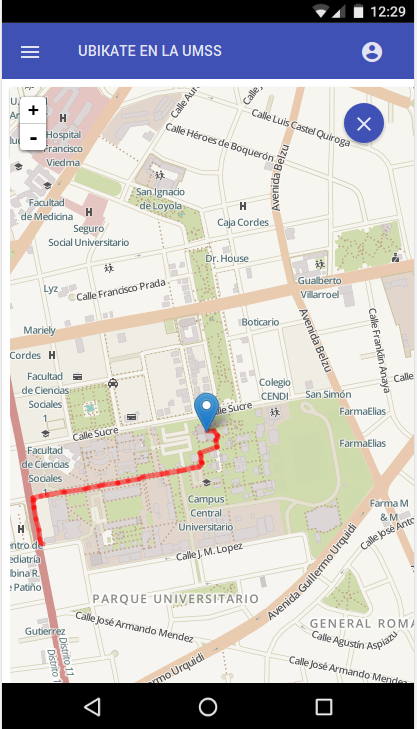
\includegraphics[width=0.5\textwidth]{iteration2/short_way_place}
    \caption{Ruta más corta dibujada con una línea roja.}
    \label{fig:short_way_place}
    \caption*{Fuente: Elaboración propia.}
  \end{center}
\end{figure}



Para dibujar líneas rectas sobre un mapa hay que tomar en consideración que la tierra no es plana y las líneas que en un mapa parecen líneas rectas, realmente no son rectas, ya que el planeta Tierra es un \emph{esferoide oblato}\footnote{Un \emph{esferoide oblato} (o elipsoide oblato) es un elipsoide de revolución obtenido por rotación de una elipse alrededor de su eje más corto.} por lo que las líneas en apariencia rectas tienen la curvatura natural del planeta Tierra. En distancias largas esto tiene un gran impacto al manejar o utilizar mapas proyectados, pero también es cierto que para una área pequeña como es el campus de la Universidad de San Simón este problema no tiene un gran impacto pero no está demás en tomar en cuenta esta característica en el análisis de datos geoespaciales, como se explicó en el capitulo \ref{cha:geolocalizacion}, para el presente proyecto se usará el proyección \emph{SRID 3857}.\\
% movido a iteration 2



% movido a iteration 2

\subsection{Manejo de Usuarios}
\label{sub:Manejo de Usuarios}

Si se quiere saber la ruta más corta entre el usuario y un lugar conocer la locación del usuario, hay que tomar en cuenta que esta información no se encuentra en la base de datos, es necesario obtener el punto georreferenciado del usuario como punto de inicio, para lo cual se utilizó el API de geolocalización propio de HTML5, la especificación de HTML5 indica que el navegador puede acceder y usar los recursos nativos de un smartphone pero es necesaria la aceptación del usuario mediante un mensaje que el navegador despliega, la locación es encontrada mediante la triangulación de Coordenadas por GPS (el mas exacto a la hora de encontrar la locación del dispositivo), Wi-Fi, GSM o CDMA. Solo es necesaria la ejecución de la siguiente línea para poder obtener la posición actual del usuario usando el API de geolocalización de HTML5. \\

\begin{verbatim}
  var coords = Geolocation.getCurrentPosition();
  var latitud = coords.latitude;
  var longitud = coords.longitude;
\end{verbatim}

La \emph{latitud} y \emph{longitud} obtenidas es fácilmente trasladado al mapa usando \emph{ember-leaflet} mediante un marcador, como se puede apreciar en la siguiente figura.

\begin{figure}[H]
  \begin{center}
    \caption{Tooltip con la latitud y longitud de la posición actual del usuario.}
    \label{fig:location_marker}
    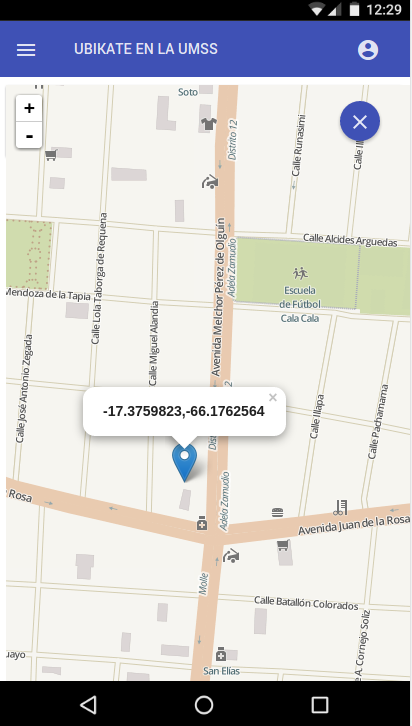
\includegraphics[width=0.5\textwidth]{iteration2/location_marker}
    \caption*{Fuente: Elaboración propia.}
  \end{center}
\end{figure}

% movido a iteration 2



\subsection{Informe de los datos}
\label{sub:Informe de los datos}
